\documentclass[twoside]{article}


\usepackage[sc]{mathpazo} % Use the Palatino font
\usepackage[T1]{fontenc} % Use 8-bit encoding that has 256 glyphs
\linespread{1.3} % Line spacing - Palatino needs more space between lines
\usepackage{microtype} % Slightly tweak font spacing for aesthetics

\usepackage[hmarginratio=1:1,top=32mm,columnsep=20pt]{geometry} % Document margins
\usepackage{multicol} % Used for the two-column layout of the document
\usepackage[hang, small,labelfont=bf,up,textfont=it,up]{caption} % Custom captions under/above floats in tables or figures
\usepackage{booktabs} % Horizontal rules in tables
\usepackage{float} % Required for tables and figures in the multi-column environment - they need to be placed in specific locations with the [H] (e.g. \begin{table}[H])
\usepackage{hyperref} % For hyperlinks in the PDF

\usepackage{lettrine} % The lettrine is the first enlarged letter at the beginning of the text
\usepackage{paralist} % Used for the compactitem environment which makes bullet points with less space between them

\usepackage{titlesec} % Allows customization of titles
\renewcommand\thesection{\Roman{section}} % Roman numerals for the sections
\renewcommand\thesubsection{\Roman{subsection}} % Roman numerals for subsections
\titleformat{\section}[block]{\large\scshape\centering}{\thesection.}{1em}{} % Change the look of the section titles
\titleformat{\subsection}[block]{\large}{\thesubsection.}{1em}{} % Change the look of the section titles

\usepackage{fancyhdr} % Headers and footers
\pagestyle{fancy} % All pages have headers and footers
\fancyhead{} % Blank out the default header
\fancyfoot{} % Blank out the default footer
\fancyhead[C]{USC EE483} % Custom header text
\fancyfoot[RO,LE]{\thepage} % Custom footer text



\usepackage{multicol}
\usepackage{listings}
\usepackage{graphicx}
\usepackage{caption}
\usepackage{subcaption}
\usepackage{hyperref}
\usepackage{color}
\usepackage{float}
\usepackage{mathtools}
\usepackage{amssymb}
\usepackage{wrapfig}


\lstset{ %
language=Matlab,                % choose the language of the code
basicstyle=\footnotesize,       % the size of the fonts that are used for the code
numbers=left,                   % where to put the line-numbers
numberstyle=\footnotesize,      % the size of the fonts that are used for the line-numbers
stepnumber=1,                   % the step between two line-numbers. If it is 1 each line will be numbered
numbersep=5pt,                  % how far the line-numbers are from the code
backgroundcolor=\color{white},  % choose the background color. You must add \usepackage{color}
showspaces=false,               % show spaces adding particular underscores
showstringspaces=false,         % underline spaces within strings
showtabs=false,                 % show tabs within strings adding particular underscores
frame=single,           % adds a frame around the code
tabsize=2,          % sets default tabsize to 2 spaces
captionpos=b,           % sets the caption-position to bottom
breaklines=true,        % sets automatic line breaking
breakatwhitespace=false,    % sets if automatic breaks should only happen at whitespace
escapeinside={\%*}{*)}          % if you want to add a comment within your code
}
%----------------------------------------------------------------------------------------
%	TITLE SECTION
%----------------------------------------------------------------------------------------

\title{\vspace{-15mm}\fontsize{24pt}{10pt}\selectfont\textbf{Project \#4 - Integrals and Intervals }} % Article title

\author{
\large
\textsc{Li Yicheng}\thanks{\href{https://github.com/IAMLYCHEE/EE483}{github link: https://github.com/IAMLYCHEE/EE483} }\\[2mm] % Your name
\normalsize USCID:7827077047\\
\normalsize email: l.y.c.liyicheng@gmail.com \\ % Your institution
\normalsize USC Viterbi of Engineering
\vspace{-5mm}
}

\date{}

%----------------------------------------------------------------------------------------

\begin{document}

\maketitle % Insert title

\thispagestyle{fancy} % All pages have headers and footers
% \begin{multicols*}{2}
\noindent \textbf {2(a)}\\
\begin{figure}[H]
   \centering
   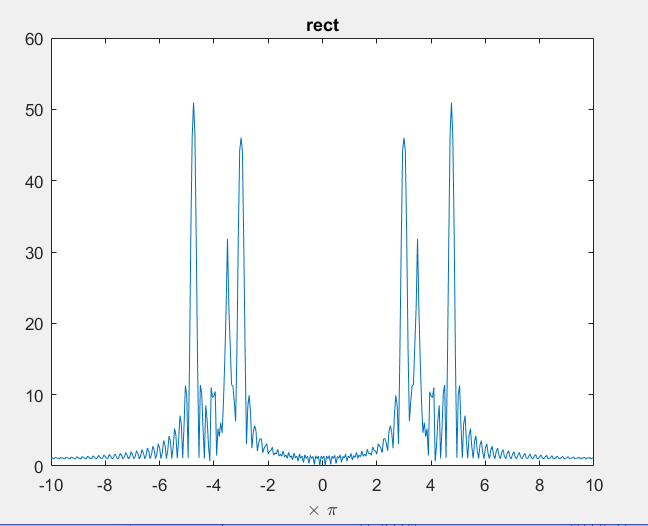
\includegraphics[width = 0.5\textwidth]{./data/rect.png}  
   \caption{DFT spectral estimation}
\end{figure}
The spectral peaks at 3, 3.5 , 4.75 can be seen however we may not tell if at 4$\pi$, it is a peak or a sidelobe.\\
\noindent \textbf {2(b)}\\
\begin{figure}[H]
   \centering
   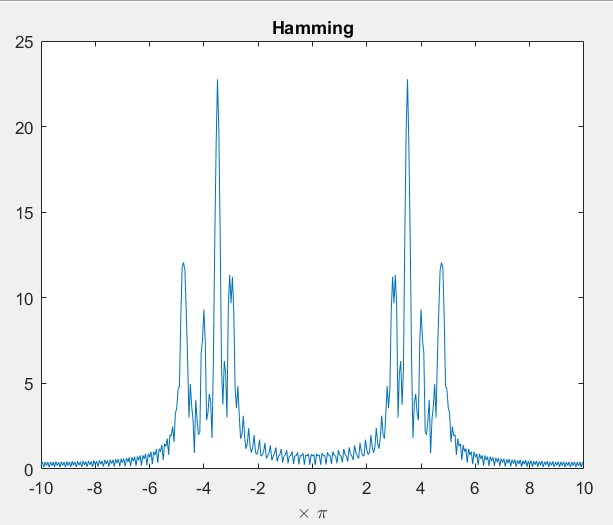
\includegraphics[width = 0.5\textwidth]{./data/hamming.png}  
   \caption{Hamming}
\end{figure}
\begin{figure}[H]
   \centering
   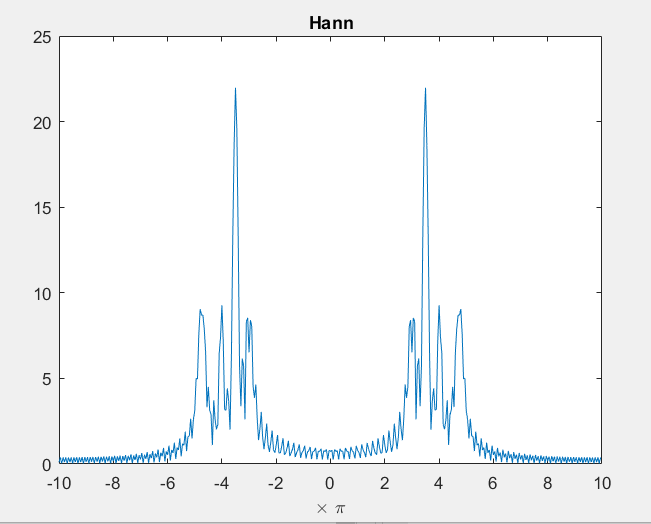
\includegraphics[width = 0.5\textwidth]{./data/hann.png}  
   \caption{Hann}
\end{figure}
\begin{figure}[H]
   \centering
   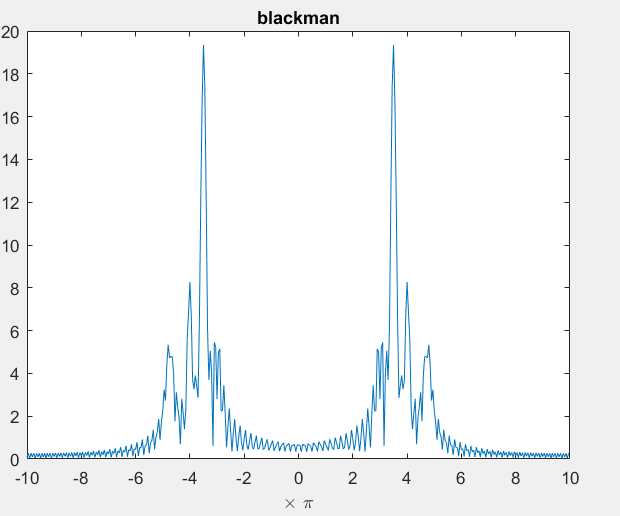
\includegraphics[width = 0.5\textwidth]{./data/blackman.png}  
   \caption{Blackman}
\end{figure}
Hamming window performs best to distinguish 4 peaks however, after appling these windows, the amplitude characteristic of the original signal may be eliminated.\\ 

\noindent \textbf {2(c)  100 Hz}
results:(the x axis is scaled from frequency from -10$\pi$ to 10$\pi$):
\begin{figure}[H]
   \centering
   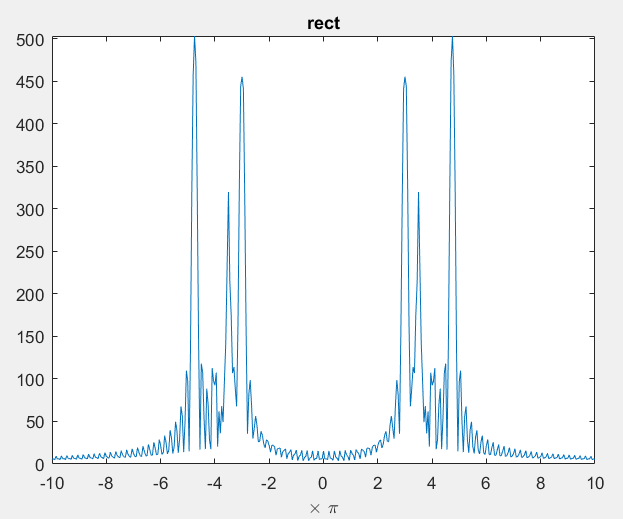
\includegraphics[width = 0.5\textwidth]{./data/rect_100.png}  
   \caption{}
\end{figure}
\begin{figure}[H]
   \centering
   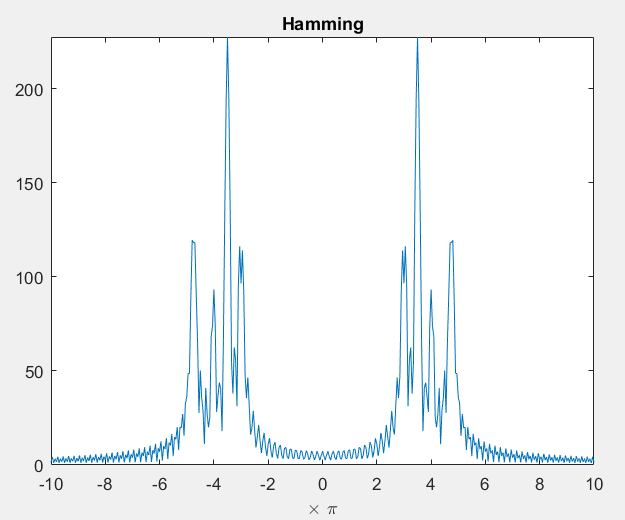
\includegraphics[width = 0.5\textwidth]{./data/hamming_100.png}  
   \caption{Hamming}
\end{figure}
\begin{figure}[H]
   \centering
   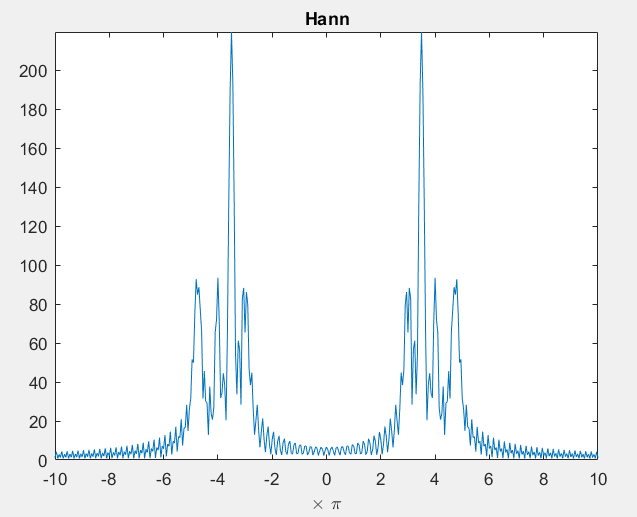
\includegraphics[width = 0.5\textwidth]{./data/hann_100.png}  
   \caption{Hann}
\end{figure}
\begin{figure}[H]
   \centering
   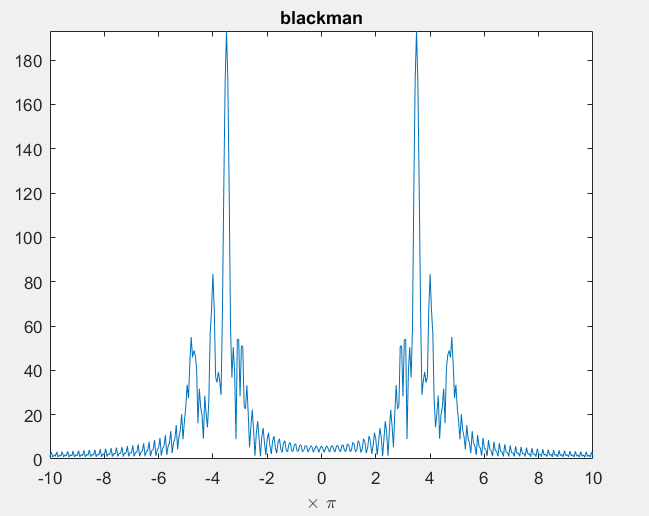
\includegraphics[width = 0.5\textwidth]{./data/blackman_100.png}  
   \caption{Blackman}
\end{figure}
If compared to the figures got with 10 Hz sampling, the 100 Hz sampling ones actually did not lead to improvements in the spectral estimation. Although it has effect on the amplitude bowever such effects also applied on sidelobe.\\

\noindent \textbf {2(d)}\\
\begin{figure}[H]
   \centering
   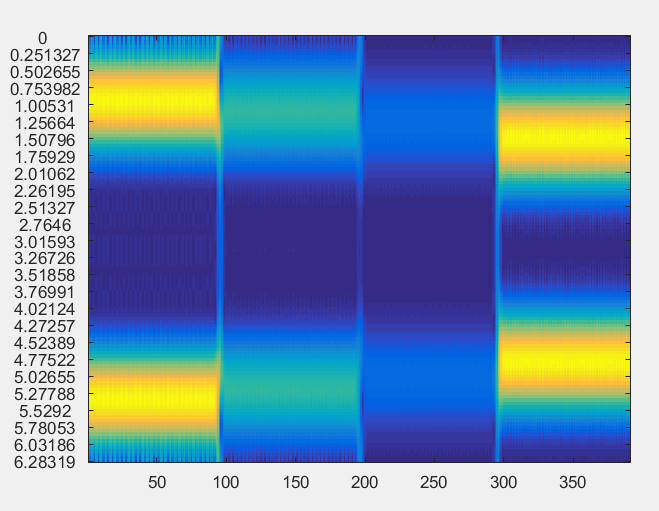
\includegraphics[width = 0.5\textwidth]{./data/2(d).png}  
   \caption{STFT}
\end{figure}
Yes, the images shows the feature of the giving signal,that its frequency is getting higher and in every 10 ten second the frequency remains the same.\\

\noindent \textbf {appendix: code}
\noindent \textbf {2(a)(b)}
\begin{lstlisting}
clear
%a
fs = 100;
t = 0 : 1/fs : 40-1/fs;
N = length(t);
index = t * fs;
signal = cos(3 * pi * t) .* (t < 10) +...
    1/2 * sin(3.5 * pi * t) .* (t >= 10 & t < 20)+...
    1/6 * cos(4 * pi * t) .* (t >= 20 & t < 30) +...
    sin(4.75 * pi * t) .* (t >= 30 & t < 40);
X = fft(signal);
t = (index - N/2)/ N * fs * 2;
plot(t,abs(fftshift(X)))
xlabel('\times \pi')
axis([-10 10 0 max(abs(X))])
title('rect')
%b
%hamming
window = hamming(N);
x = signal .* window';
X = fft(x);
t = (index - N/2)/ N * fs * 2;
figure
plot(t,abs(fftshift(X)));
xlabel('\times \pi')
axis([-10 10 0 max(abs(X))])
title('Hamming')

%hann
window = hann(N);
x = signal .* window';
X = fft(x);
t = (index - N/2)/ N * fs * 2;
figure
plot(t,abs(fftshift(X)))
xlabel('\times \pi')
axis([-10 10 0 max(abs(X))])
title('Hann')

%blackman
window = blackman(N);
x = signal .* window';
X = fft(x);
t = (index - N/2)/ N * fs * 2;
figure
plot(t,abs(fftshift(X)))
xlabel('\times \pi')
axis([-10 10 0 max(abs(X))])
title('blackman')
\end{lstlisting}
\noindent \textbf {2(c)}
\begin{lstlisting}
clear
%a
fs = 100;
t = 0 : 1/fs : 40-1/fs;
N = length(t);
index = t * fs;
signal = cos(3 * pi * t) .* (t < 10) +...
    1/2 * sin(3.5 * pi * t) .* (t >= 10 & t < 20)+...
    1/6 * cos(4 * pi * t) .* (t >= 20 & t < 30) +...
    sin(4.75 * pi * t) .* (t >= 30 & t < 40);
X = fft(signal);
t = (index - N/2)/ N * fs * 2;
plot(t,log(abs(fftshift(X))))
xlabel('\times \pi')
title('rect')
%b
%hamming
window = hamming(N);
x = signal .* window';
X = fft(x);
t = (index - N/2)/ N * fs * 2;
figure
plot(t,log(abs(fftshift(X))))
xlabel('\times \pi')
title('Hamming')

%hann
window = hann(N);
x = signal .* window';
X = fft(x);
t = (index - N/2)/ N * fs * 2;
figure
plot(t,log(abs(fftshift(X))))
xlabel('\times \pi')
title('Hann')

%blackman
window = blackman(N);
x = signal .* window';
X = fft(x);
t = (index - N/2)/ N * fs * 2;
figure
plot(t,log(abs(fftshift(X))))
xlabel('\times \pi')
title('blackman')
\end{lstlisting}
\noindent \textbf {2(d)}
\begin{lstlisting}
clear
fs = 10;
t = 0 : 1/fs : 40-1/fs;
N = length(t);
index = t * fs;
signal = cos(3 * pi * t) .* (t < 10) +...
    1/2 * sin(3.5 * pi * t) .* (t >= 10 & t < 20)+...
    1/6 * cos(4 * pi * t) .* (t >= 20 & t < 30) +...
    sin(4.75 * pi * t) .* (t >= 30 & t < 40);
tWindow  = 1;
windowLength = fs * tWindow;
window = hamming(windowLength)';
yAmount = length(0:0.05:2*pi);
result = zeros(yAmount, N-windowLength + 1); 
for m = 0 : N - windowLength
    k = 1;
    for omega = 0 : 0.05 : 2 * pi
        index = m + 1 : m + windowLength;
        result(k,m+1)=sum(signal(index) .* window .* exp(-1i*omega*index));
        k = k + 1; %put less frequency down the axis
    end
end
imagesc(abs(result));
ytickLabels = linspace(0,2*pi,length(1:5:size(result,1)));
set(gca, 'YTick',1:5:126 , 'YTickLabel', ytickLabels)
\end{lstlisting}
% \end{multicols*}
\end{document}